\documentclass[aspectratio=169,11pt]{beamer}
\usetheme{default}\usecolortheme{seagull}\setbeamertemplate{navigation symbols}{}\setbeamertemplate{footline}{\hfill\scriptsize\insertframenumber/\inserttotalframenumber\hspace{2mm}\vspace{1mm}}
\usepackage[T1]{fontenc}\usepackage[utf8]{inputenc}\usepackage{lmodern}\usepackage{url}\usepackage{graphicx}
\setbeamerfont{frametitle}{size=\large,series=\bfseries}\setbeamercolor{frametitle}{fg=black}\setbeamertemplate{frametitle}{\vspace{2mm}\insertframetitle\par\vspace{1mm}\hrule}
\setbeamertemplate{itemize items}[circle]
\title{Off-street parking on rue de Terrebonne}\subtitle{What the 1954--55 fire-insurance plans, today's aerial imagery and the City's LiDAR show, building by building}\author{Terrebonne-open-sources (a resident of Côte-des-Neiges--Notre-Dame-de-Grâce) \quad 2026-10-25}\date{}
\begin{document}
\begin{frame}\titlepage\vfill{\tiny Source: Underwriters' Survey Bureau, Insurance plan of the city of Montreal, vol.~7, 1954--55 (BAnQ, notice 0000174390). Reading: the author, one row per building. Imagery: Gouvernement du Québec (Imagerie\_GQ, fetched Oct.~25, 2026). LiDAR: Ville de Montréal 2015, CC-BY 4.0.}\end{frame}
\begin{frame}{60\,\% of the buildings on Terrebonne were built with a garage}\begin{columns}[T]\column{0.6\textwidth}\begin{itemize}\item 126 residential buildings with a Terrebonne address, west end of the lane to Girouard, on the sixteen 1954--55 sheets available
\item 75 were built with a garage (north side 57 of 90, south side 18 of 36)
\item By dwellings (City roll): 192 of 324, 59\,\%
\item The plans mark garages, not driveways: a lower bound for ``garage or driveway as built''\end{itemize}\column{0.38\textwidth}\centering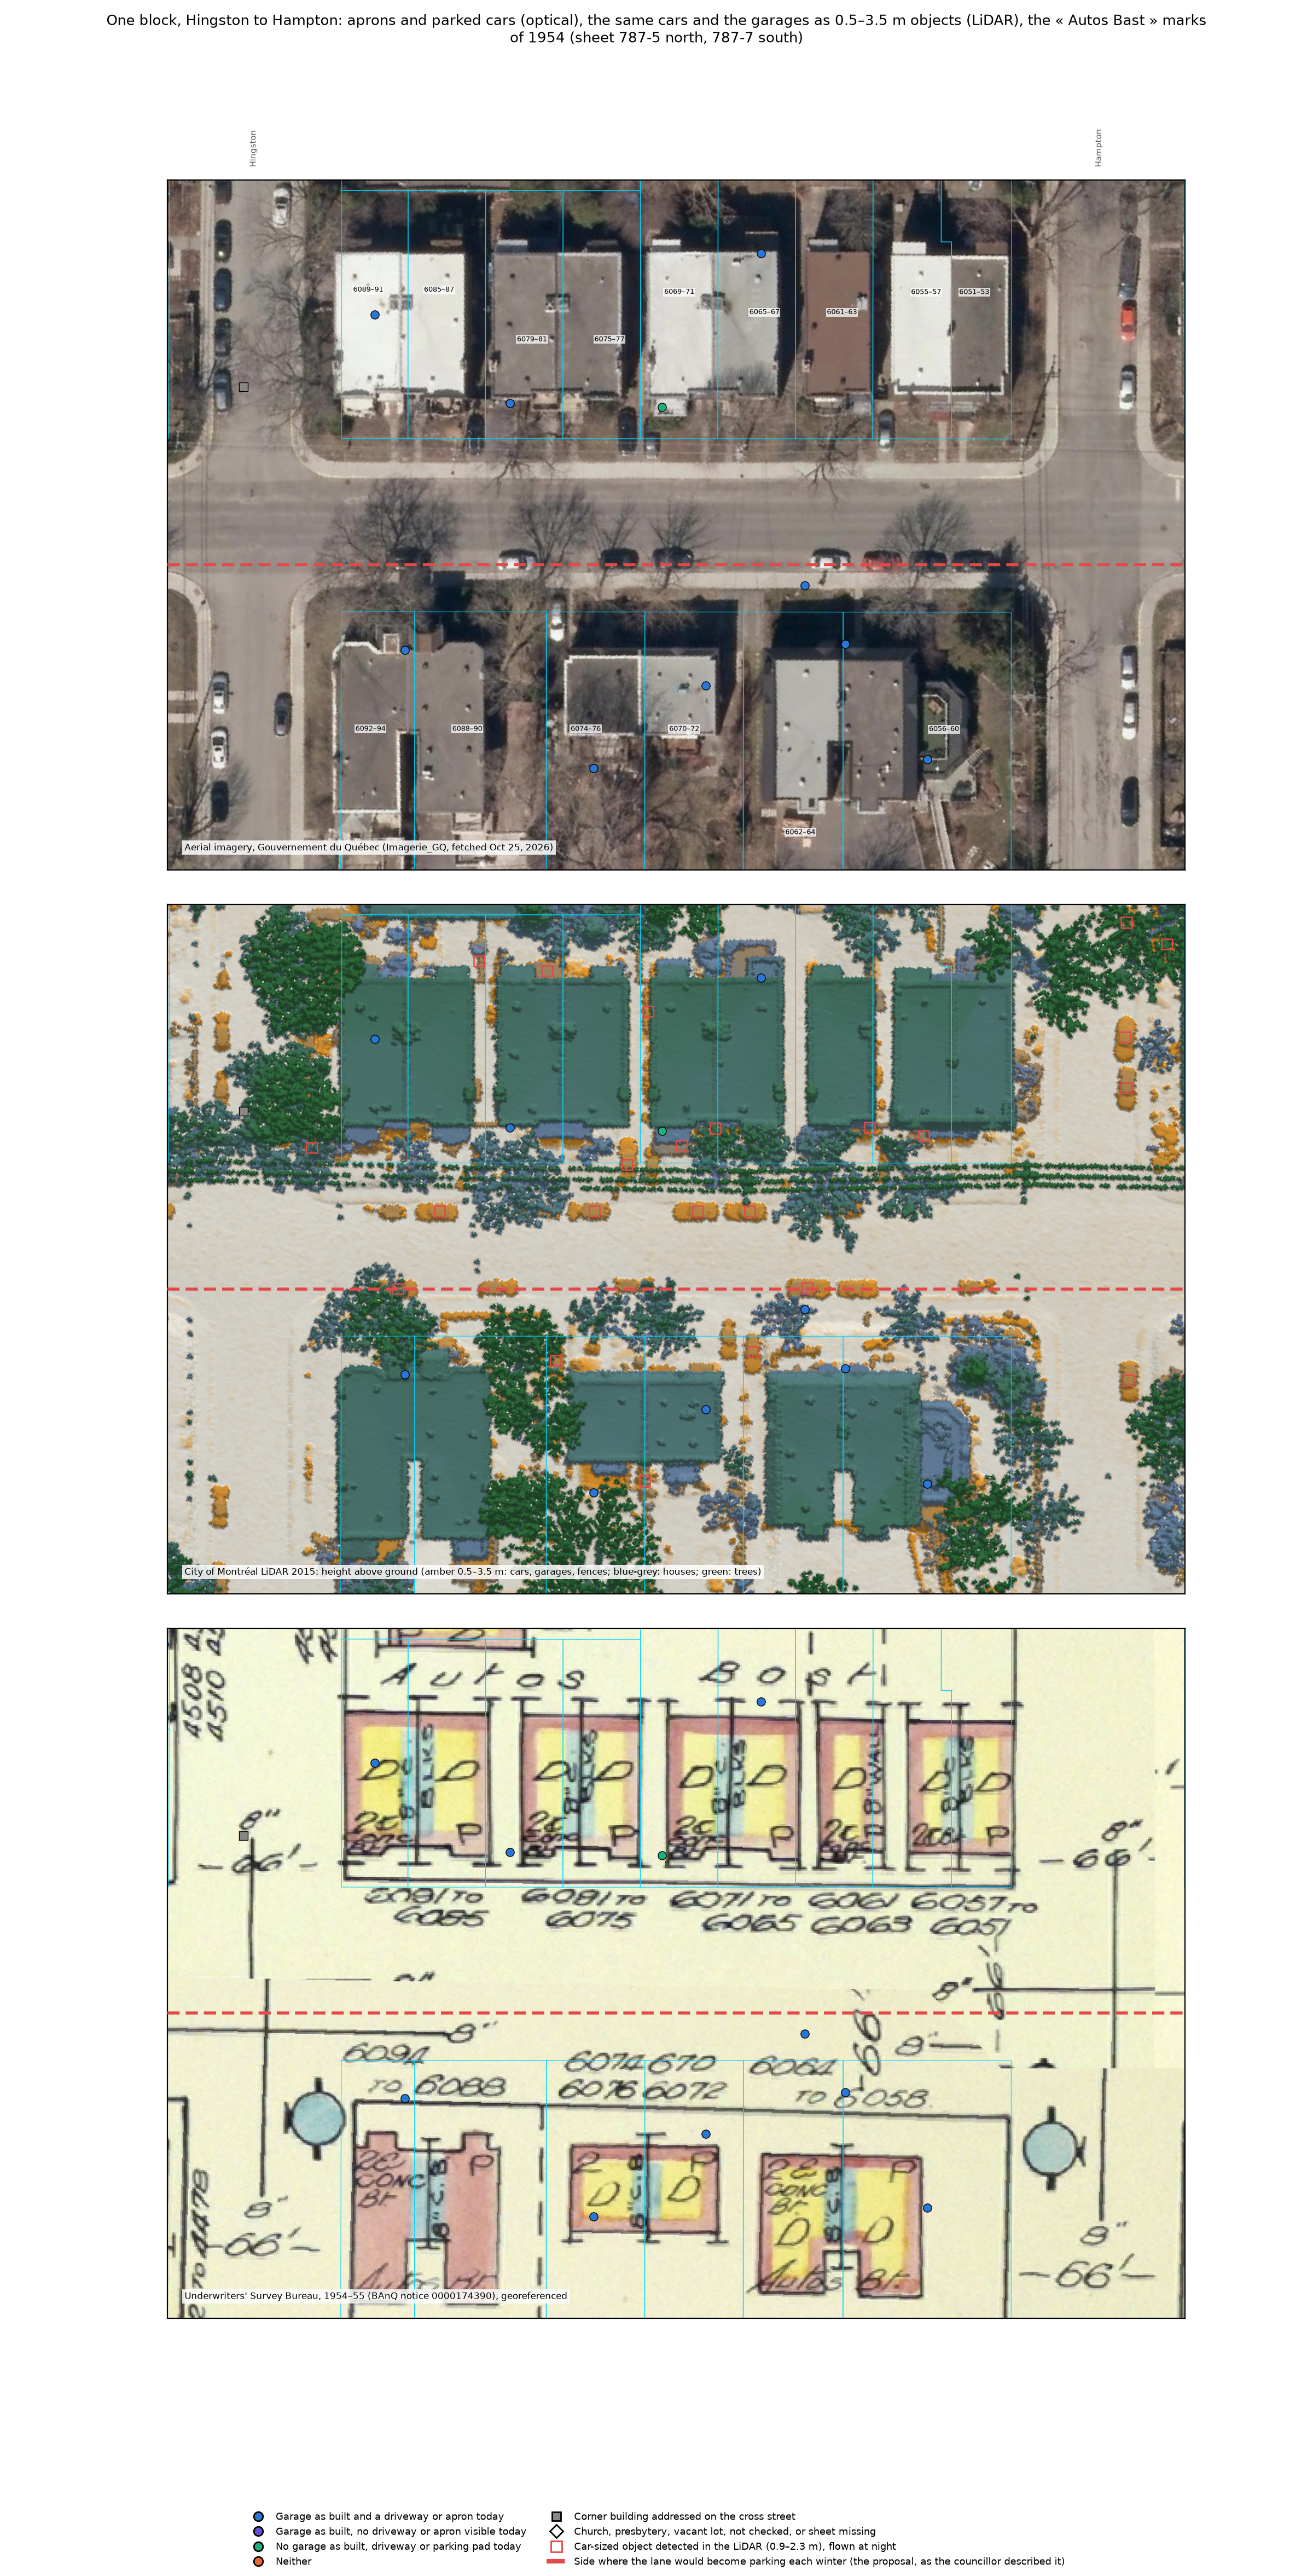
\includegraphics[height=0.68\textheight]{figures/method_detail_hingston_hampton_en.png}\end{columns}\vfill{\tiny Source: Underwriters' Survey Bureau, Insurance plan of the city of Montreal, vol.~7, 1954--55 (BAnQ, notice 0000174390). Reading: the author, one row per building.}\end{frame}
\begin{frame}{Today, 72\,\% have a garage as built or a visible driveway}\begin{itemize}\item 123 buildings checked on the Québec government's aerial imagery (leaf-off, 8\,cm per pixel, after June 2024)
\item 79 show a driveway, paved apron or parking pad today (64\,\%)
\item Garage as built \emph{or} driveway today: 89 of 123 (72\,\%); by dwellings 73\,\%
\item Of the 1954 garages, 64 keep a visible apron, 10 do not; 15 houses without a garage in 1954 have a driveway today
\item What a garage holds inside cannot be seen from above\end{itemize}\vfill{\tiny Imagery: Gouvernement du Québec (Imagerie\_GQ, fetched Oct.~25, 2026). LiDAR: Ville de Montréal 2015, CC-BY 4.0. Base: Ville de Montréal open data, CC-BY 4.0 (géobase, assessment roll). Reading: the author.}\end{frame}
\begin{frame}{Where the garages and driveways are, along the whole street}\begin{center}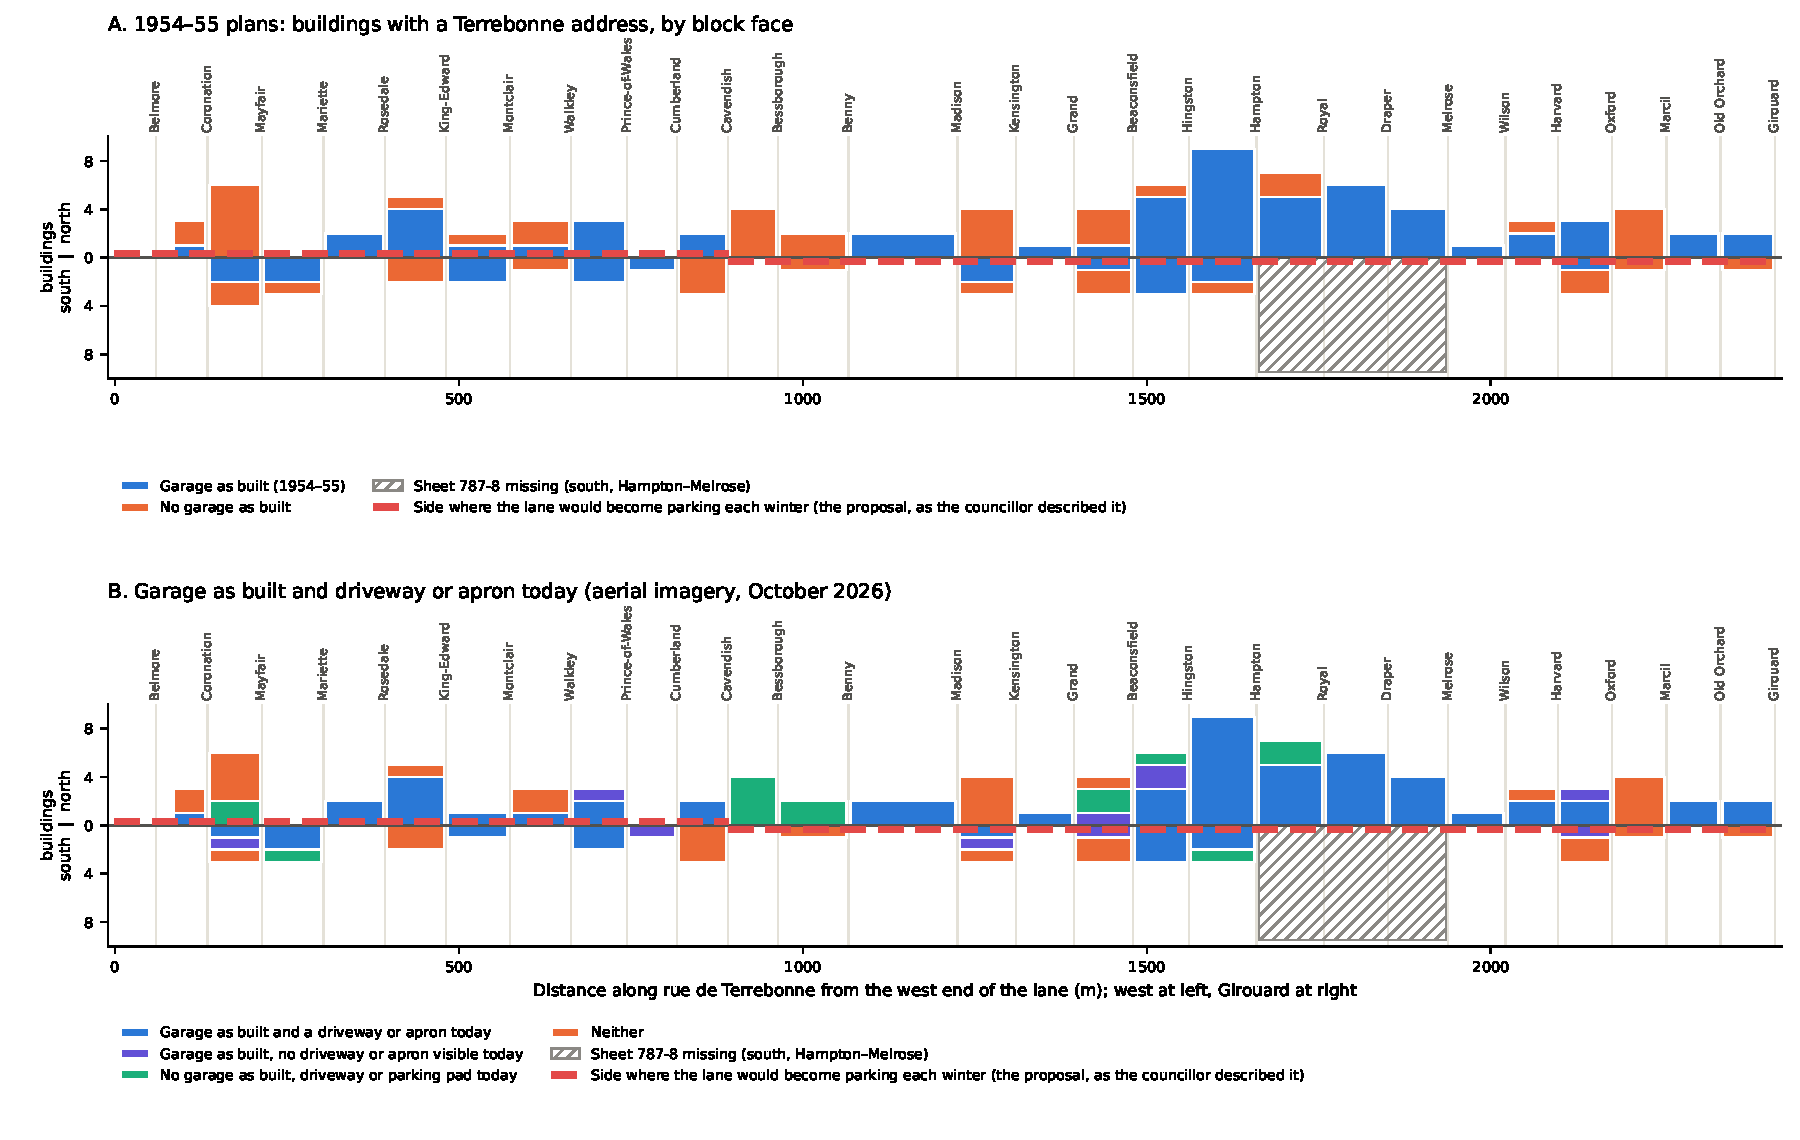
\includegraphics[height=0.72\textheight]{figures/terrebonne_garages_distribution_en.pdf}\end{center}\vfill{\scriptsize Dashed red: the side where the lane would become parking each winter under the proposal, as the councillor described it.}\\{\tiny Source: Underwriters' Survey Bureau, Insurance plan of the city of Montreal, vol.~7, 1954--55 (BAnQ, notice 0000174390). Reading: the author, one row per building. Imagery: Gouvernement du Québec (Imagerie\_GQ, fetched Oct.~25, 2026). LiDAR: Ville de Montréal 2015, CC-BY 4.0.}\end{frame}
\begin{frame}{On today's parcels: garage as built and driveway today}
\begin{center}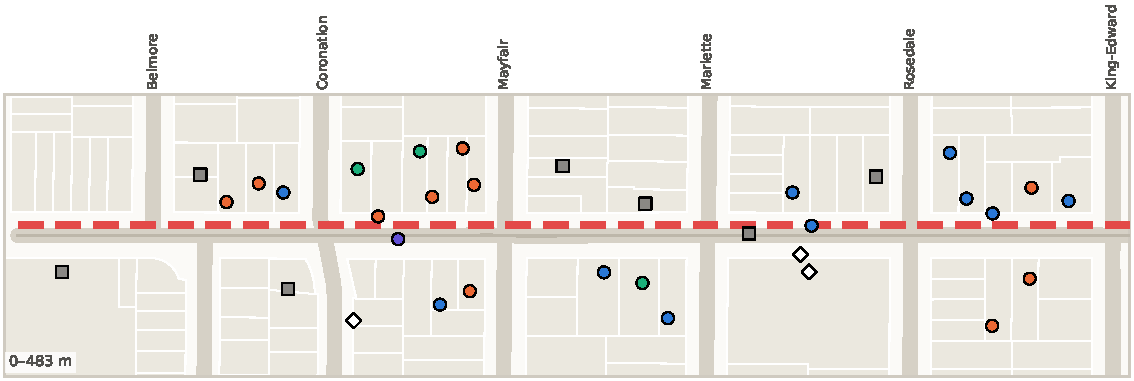
\includegraphics[width=\textwidth]{figures/panels/today_en_p1.pdf}\\[1pt]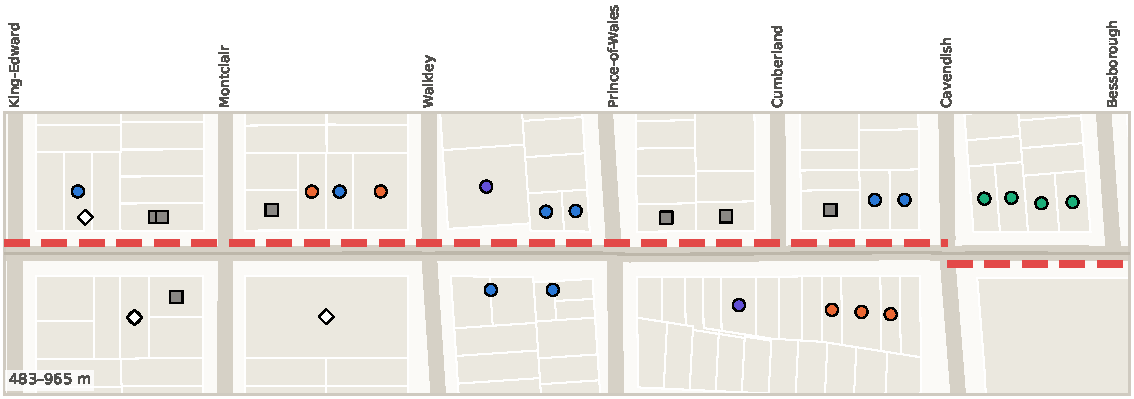
\includegraphics[width=\textwidth]{figures/panels/today_en_p2.pdf}\\[1pt]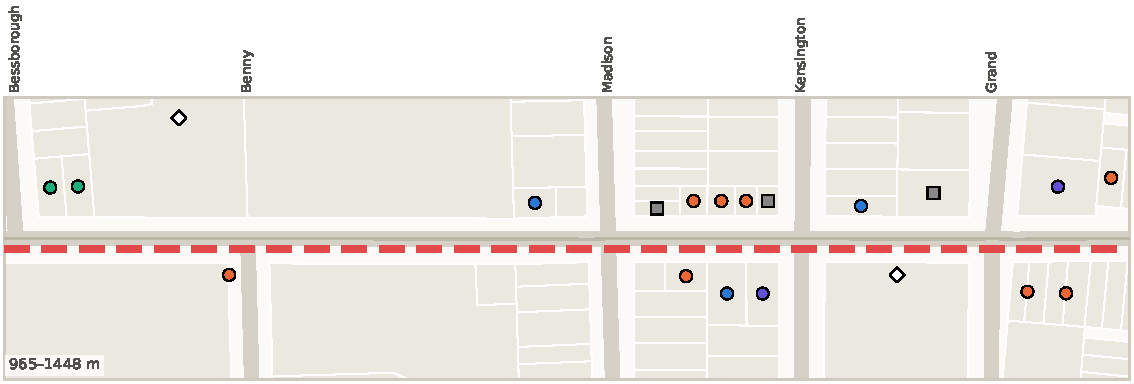
\includegraphics[width=\textwidth]{figures/panels/today_en_p3.pdf}\end{center}
\vfill{\scriptsize Dashed red: the side where the lane would become parking each winter under the proposal, as the councillor described it. \textbf{(1/2)}}\\{\tiny Base: Ville de Montréal open data, CC-BY 4.0 (géobase, assessment roll). Reading: the author. Imagery: Gouvernement du Québec (Imagerie\_GQ, fetched Oct.~25, 2026). LiDAR: Ville de Montréal 2015, CC-BY 4.0.}\end{frame}
\begin{frame}{On today's parcels: garage as built and driveway today}
\begin{center}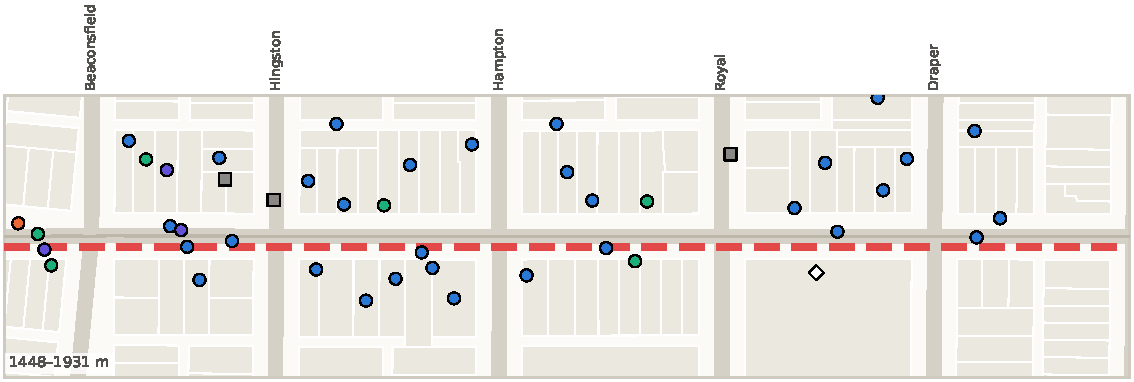
\includegraphics[width=\textwidth]{figures/panels/today_en_p4.pdf}\\[1pt]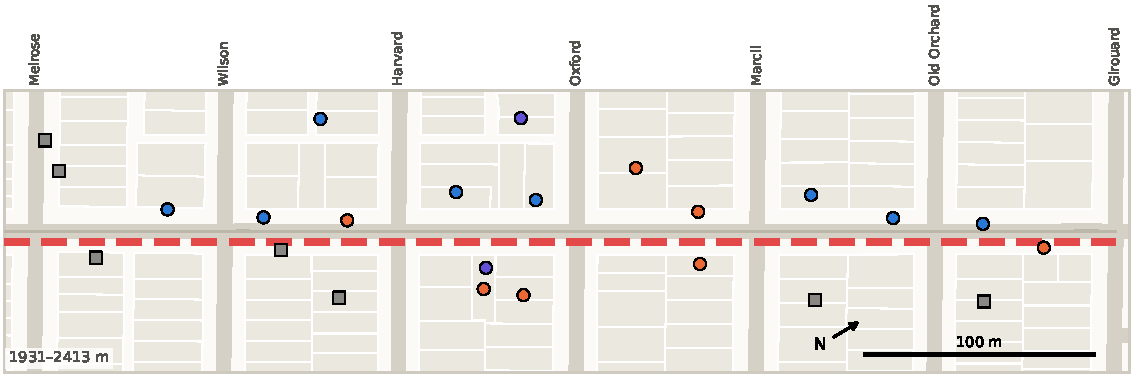
\includegraphics[width=\textwidth]{figures/panels/today_en_p5.pdf}\\[3pt]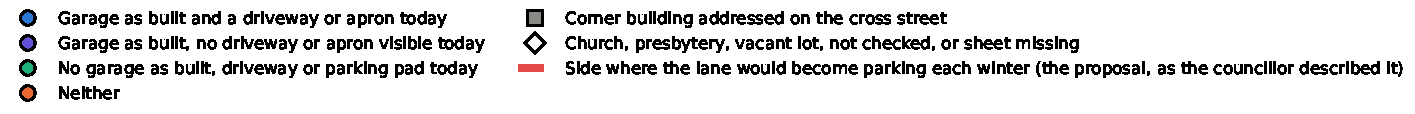
\includegraphics[width=0.95\textwidth]{figures/panels/today_en_legend.pdf}\end{center}
\vfill{\scriptsize Dashed red: the side where the lane would become parking each winter under the proposal, as the councillor described it. \textbf{(2/2)}}\\{\tiny Base: Ville de Montréal open data, CC-BY 4.0 (géobase, assessment roll). Reading: the author. Imagery: Gouvernement du Québec (Imagerie\_GQ, fetched Oct.~25, 2026). LiDAR: Ville de Montréal 2015, CC-BY 4.0.}\end{frame}
\begin{frame}{The 1954--55 plans, georeferenced: every garage is written ``Auto''}
\begin{center}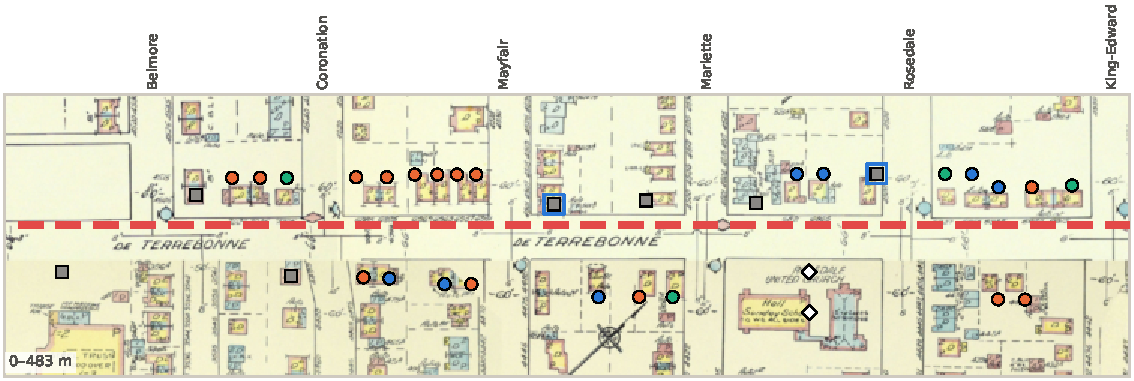
\includegraphics[width=\textwidth]{figures/panels/underwriters_en_p1.pdf}\\[1pt]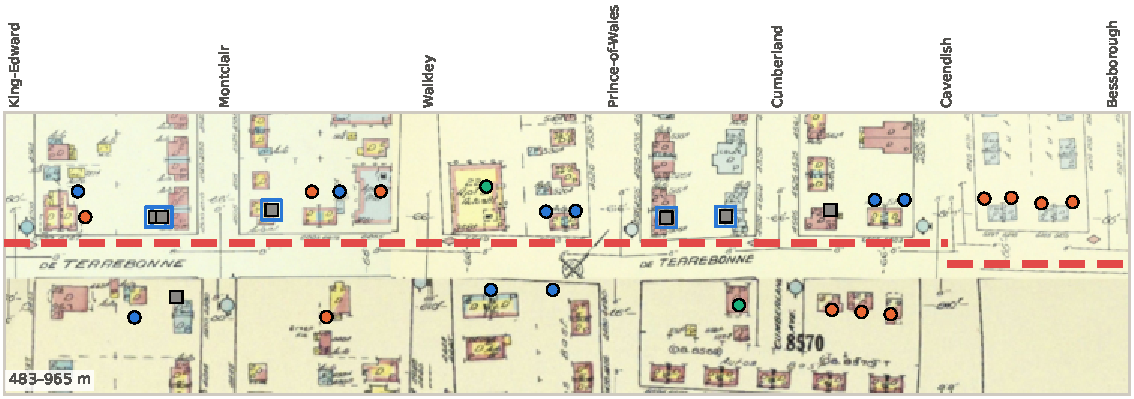
\includegraphics[width=\textwidth]{figures/panels/underwriters_en_p2.pdf}\\[1pt]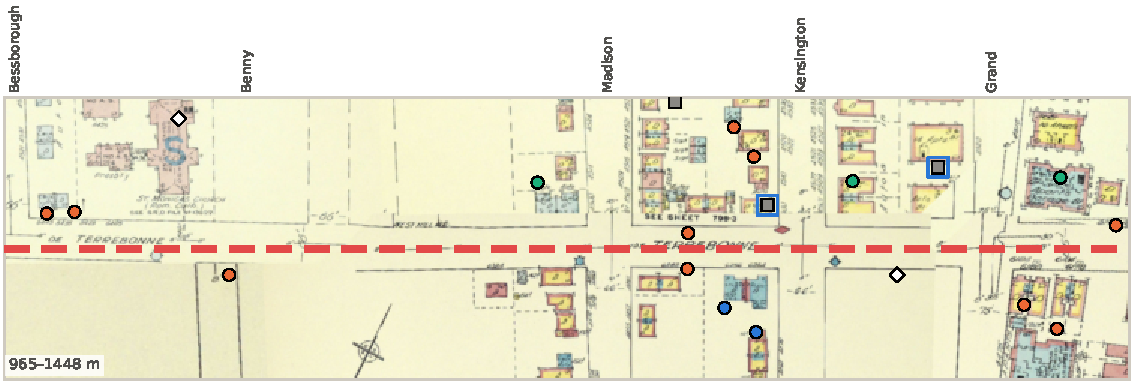
\includegraphics[width=\textwidth]{figures/panels/underwriters_en_p3.pdf}\end{center}
\vfill{\scriptsize The frontage strips of the sheets, straightened along the street; one marker per building (the blank: sheet 787-8, missing from the series). \textbf{(1/2)}}\\{\tiny Source: Underwriters' Survey Bureau, Insurance plan of the city of Montreal, vol.~7, 1954--55 (BAnQ, notice 0000174390). Reading: the author, one row per building.}\end{frame}
\begin{frame}{The 1954--55 plans, georeferenced: every garage is written ``Auto''}
\begin{center}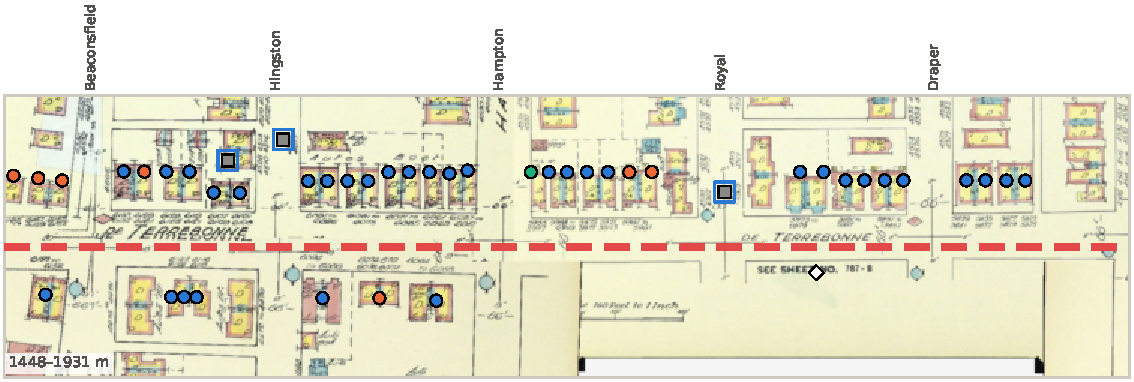
\includegraphics[width=\textwidth]{figures/panels/underwriters_en_p4.pdf}\\[1pt]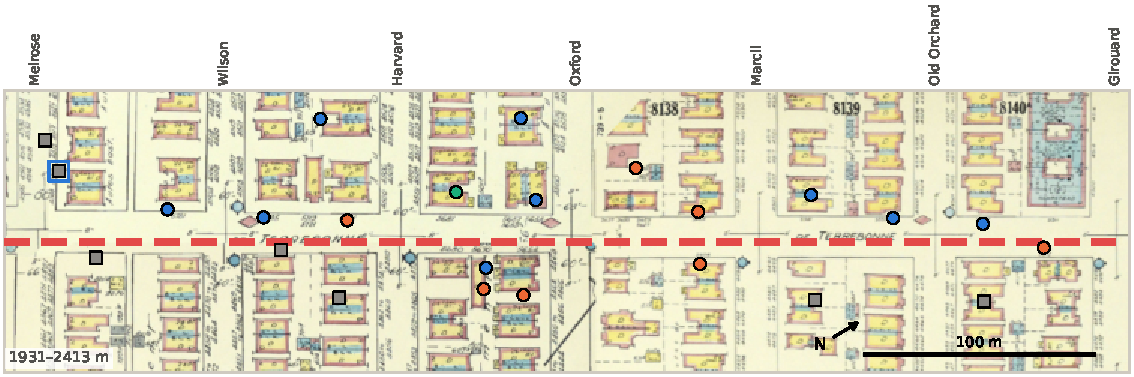
\includegraphics[width=\textwidth]{figures/panels/underwriters_en_p5.pdf}\\[3pt]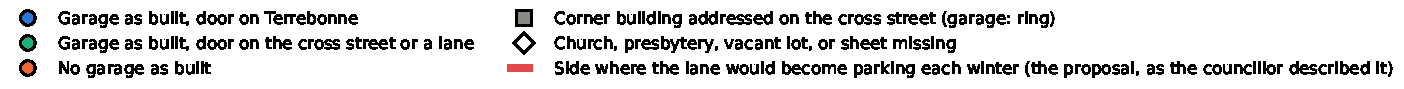
\includegraphics[width=0.95\textwidth]{figures/panels/underwriters_en_legend.pdf}\end{center}
\vfill{\scriptsize The frontage strips of the sheets, straightened along the street; one marker per building (the blank: sheet 787-8, missing from the series). \textbf{(2/2)}}\\{\tiny Source: Underwriters' Survey Bureau, Insurance plan of the city of Montreal, vol.~7, 1954--55 (BAnQ, notice 0000174390). Reading: the author, one row per building.}\end{frame}

\begin{frame}{Three sources, one frame}\begin{center}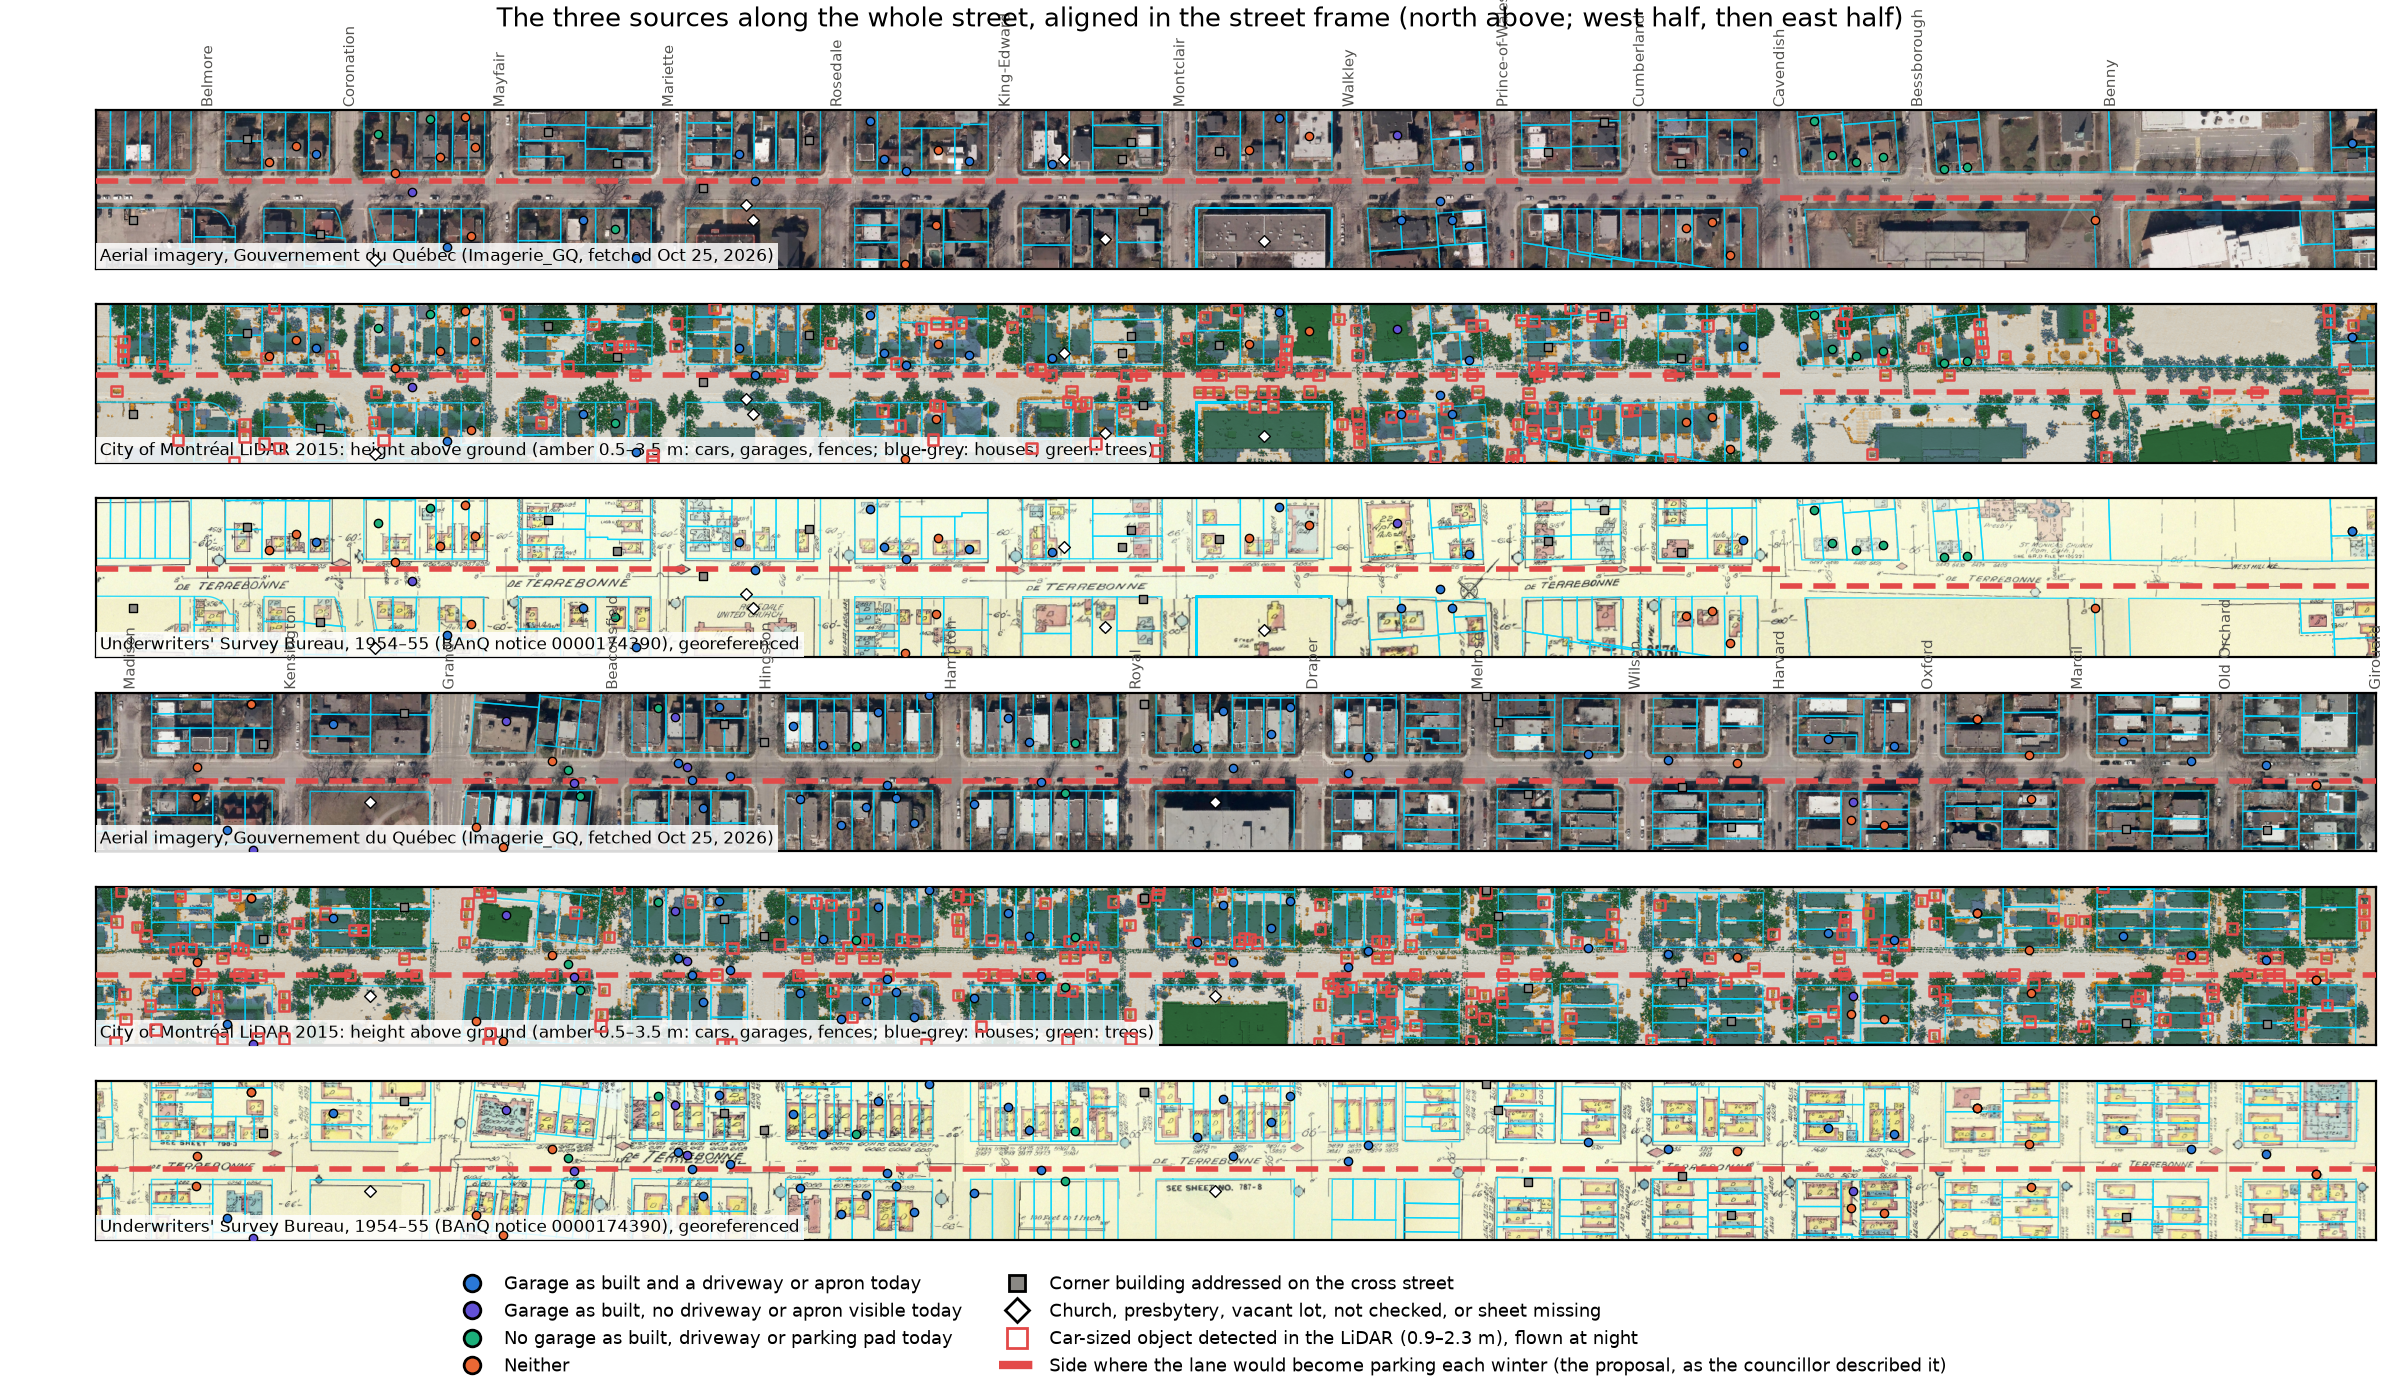
\includegraphics[height=0.74\textheight]{figures/method_overview_en.png}\end{center}\vfill{\scriptsize Aerial imagery (optical), the City's 2015 LiDAR as height above ground, and the 1954--55 sheets, all georeferenced into the same street frame.}\\{\tiny Imagery: Gouvernement du Québec (Imagerie\_GQ, fetched Oct.~25, 2026). LiDAR: Ville de Montréal 2015, CC-BY 4.0. Source: Underwriters' Survey Bureau, Insurance plan of the city of Montreal, vol.~7, 1954--55 (BAnQ, notice 0000174390). Reading: the author, one row per building.}\end{frame}
\begin{frame}{One block in the three sources: Hingston to Hampton}\begin{columns}[T]\column{0.42\textwidth}\centering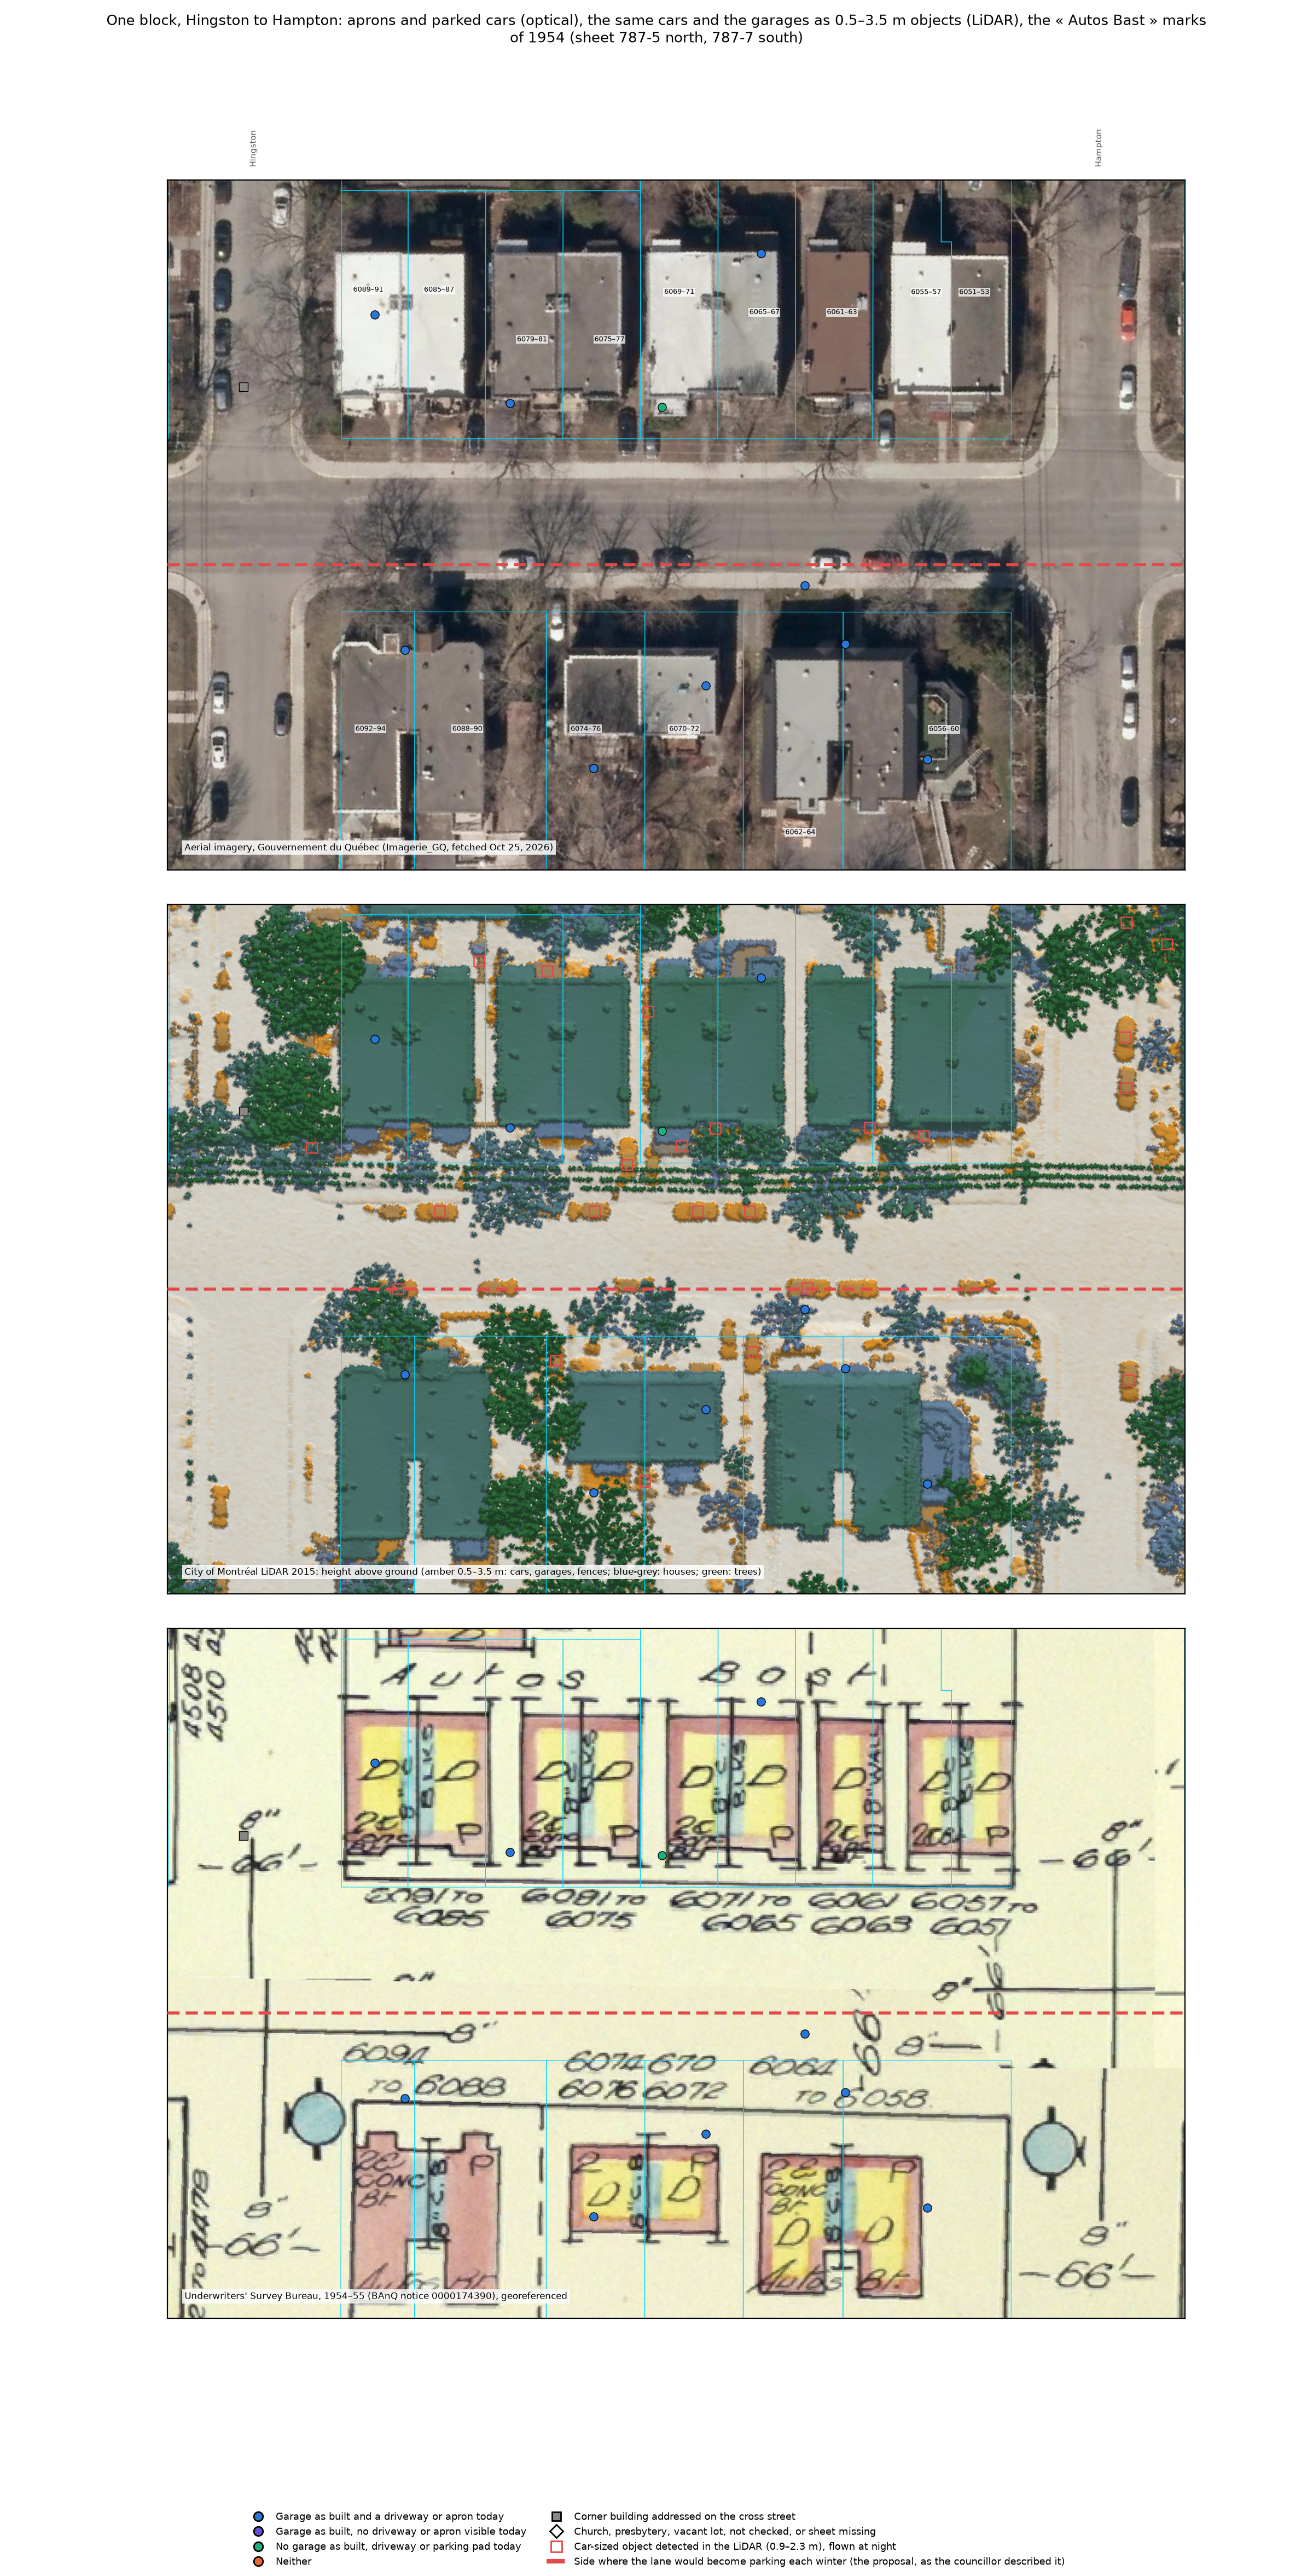
\includegraphics[height=0.74\textheight]{figures/method_detail_hingston_hampton_en.png}\column{0.56\textwidth}{\small Aprons and parked cars (optical); the same cars and the garages as 0.5--3.5\,m objects (LiDAR, red squares = automatic car detections); the ``Autos Bast'' of 1954.}\end{columns}\vfill{\tiny Imagery: Gouvernement du Québec (Imagerie\_GQ, fetched Oct.~25, 2026). LiDAR: Ville de Montréal 2015, CC-BY 4.0. Source: Underwriters' Survey Bureau, Insurance plan of the city of Montreal, vol.~7, 1954--55 (BAnQ, notice 0000174390). Reading: the author, one row per building.}\end{frame}
\begin{frame}{Cars parked on the street: two acquisitions, two moments}\begin{columns}[T]\column{0.45\textwidth}\begin{itemize}\item Daytime, spring, after June 2024 (aerial imagery): 158 cars on Terrebonne (north 30, south 128)
\item Night, 2015, before the lane (City LiDAR, 00:00--04:00): 85 cars on Terrebonne (north 38, south 47), 253 on private lots within 45\,m, 70 on the cross streets
\item Ten years and a redesign apart: each describes its moment, not a before-and-after\end{itemize}\column{0.55\textwidth}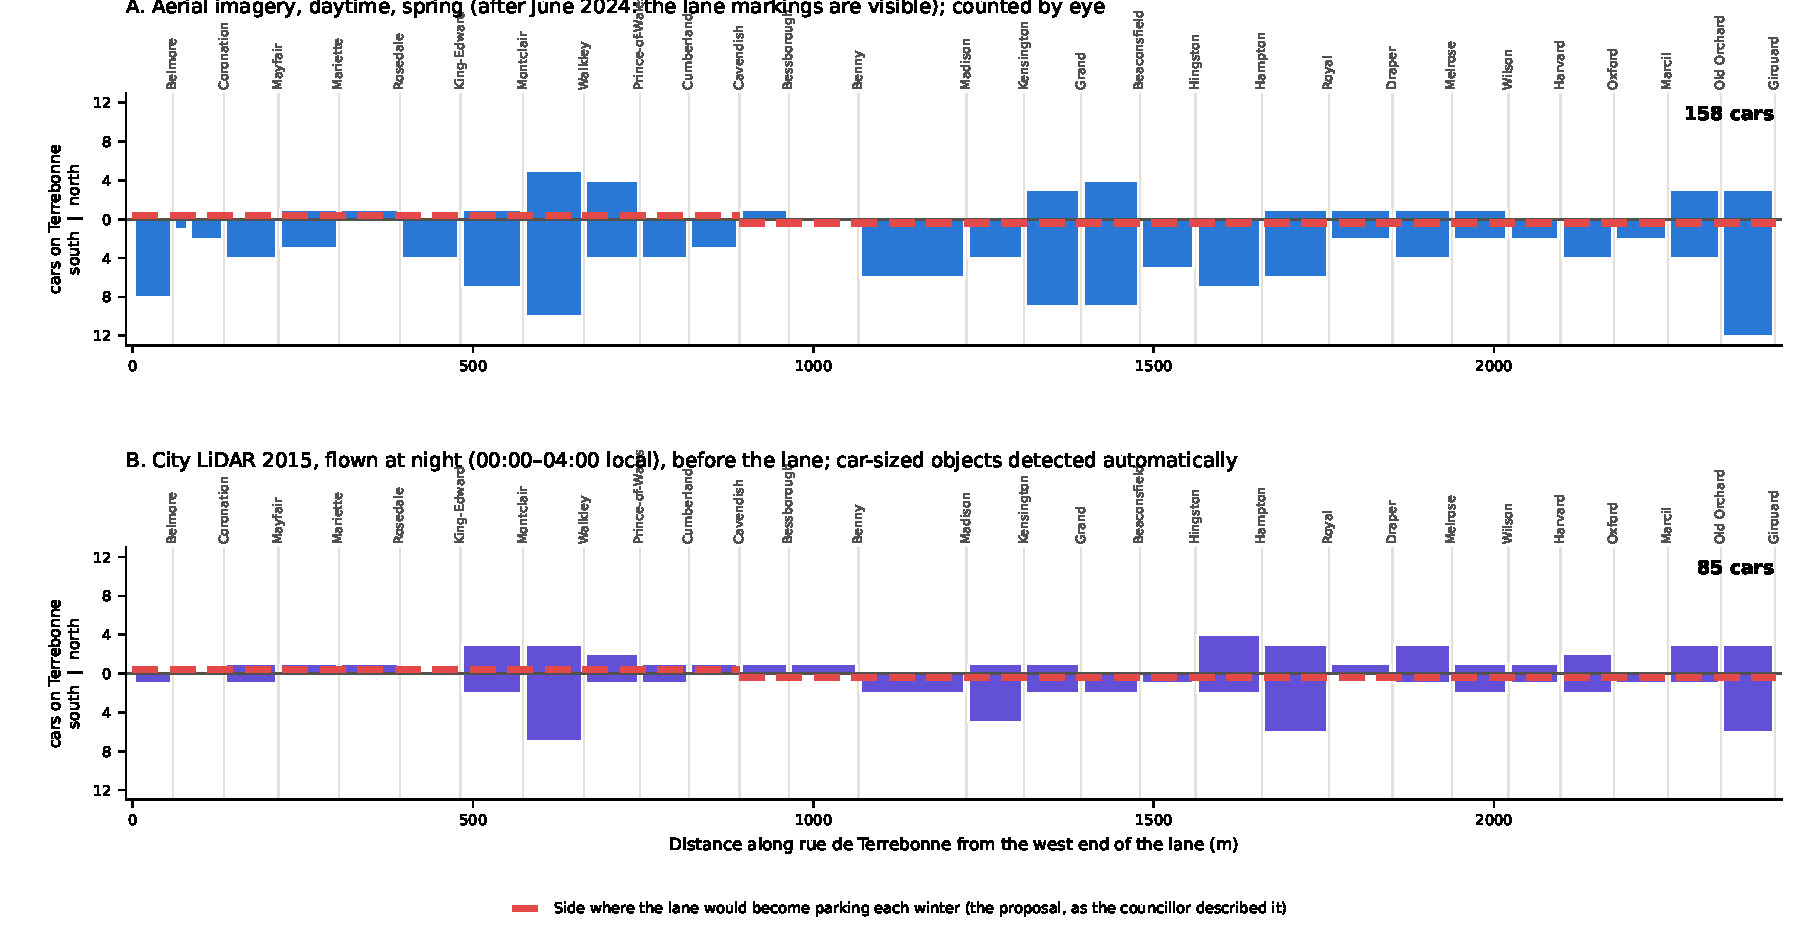
\includegraphics[width=\textwidth]{figures/terrebonne_on_street_cars_en.pdf}\end{columns}\vfill{\tiny Imagery: Gouvernement du Québec (Imagerie\_GQ, fetched Oct.~25, 2026). LiDAR: Ville de Montréal 2015, CC-BY 4.0.}\end{frame}
\begin{frame}{Caveats}\begin{itemize}\item Garages as built, not driveways: the 1954--55 share is a lower bound
\item As built, as visible: neither reading sees inside a garage (workshop, storage, living space); a 1930 garage may be too small for today's vehicles
\item Buildings, not households: a duplex pair has two to four flats and one or two garages
\item One sheet missing in 1954--55 (south side, Hampton to Melrose); readings graded medium or unclear are flagged row by row
\item Everything is in the table: one row per building, checkable by address\end{itemize}\end{frame}
\begin{frame}{Where to find it}\begin{itemize}\item Web page, note, maps, tables: \url{https://openmobilitydata.github.io/Terrebonne-open-sources/1954-underwriters-plans-terrebonne-garages/}
\item The sheets themselves: BAnQ numérique, \url{https://collections.banq.qc.ca/ark:/52327/2244199}
\item Repository: \url{https://github.com/OpenMobilityData/Terrebonne-open-sources}\end{itemize}\vfill{\tiny Source: Underwriters' Survey Bureau, Insurance plan of the city of Montreal, vol.~7, 1954--55 (BAnQ, notice 0000174390). Reading: the author, one row per building. Base: Ville de Montréal open data, CC-BY 4.0 (géobase, assessment roll). Reading: the author. Imagery: Gouvernement du Québec (Imagerie\_GQ, fetched Oct.~25, 2026). LiDAR: Ville de Montréal 2015, CC-BY 4.0.}\end{frame}
\end{document}
